\lstdefinelanguage{plaintext}{
  sensitive=false,
  comment=[l]{//},
  morecomment=[s]{/*}{*/},
  identifierstyle=\color{black},
  morestring=[b]',
  morestring=[b]"
}

\lstset
{ 
    language=plaintext,
    basicstyle=\footnotesize,
    numbers=left,
    stepnumber=1,
    showstringspaces=false,
    tabsize=1,
    breaklines=true,
    breakatwhitespace=false,
    frame=leftline
}

\chapter{Analisis}
\label{chap:analisis}

Pada bab ini dijelaskan mengenai analisis aplikasi sejenis, analisis penggunaan JGit, analisis penggunaan Selenium WebDriver, analisis penggunaan Apache Commons CLI, dan prapengujian. 

\section{Analisisi Aplikasi Sejenis}
\label{sec:analisis_aplikasi_sejenis}
Saat skripsi ini dibuat, aplikasi sejenis yang digunakan untuk membangkitkan animasi \textit{timelapse} adalah Gource.  
Proyek perangkat lunak ditampilkan oleh Gource sebagai animasi pohon, dimana pusatnya adalah \textit{root directory} dari proyek perangkat lunak\cite{Gource}. Direktori ditampilkan sebagai \textit{branch}, sedangkan \textit{file} ditampilkan sebagai \textit{leaf}. Developer dapat terlihat di \textit{working tree} pada saat mereka berkontribusi untuk proyek.

\begin{figure}[H]
	\centering
		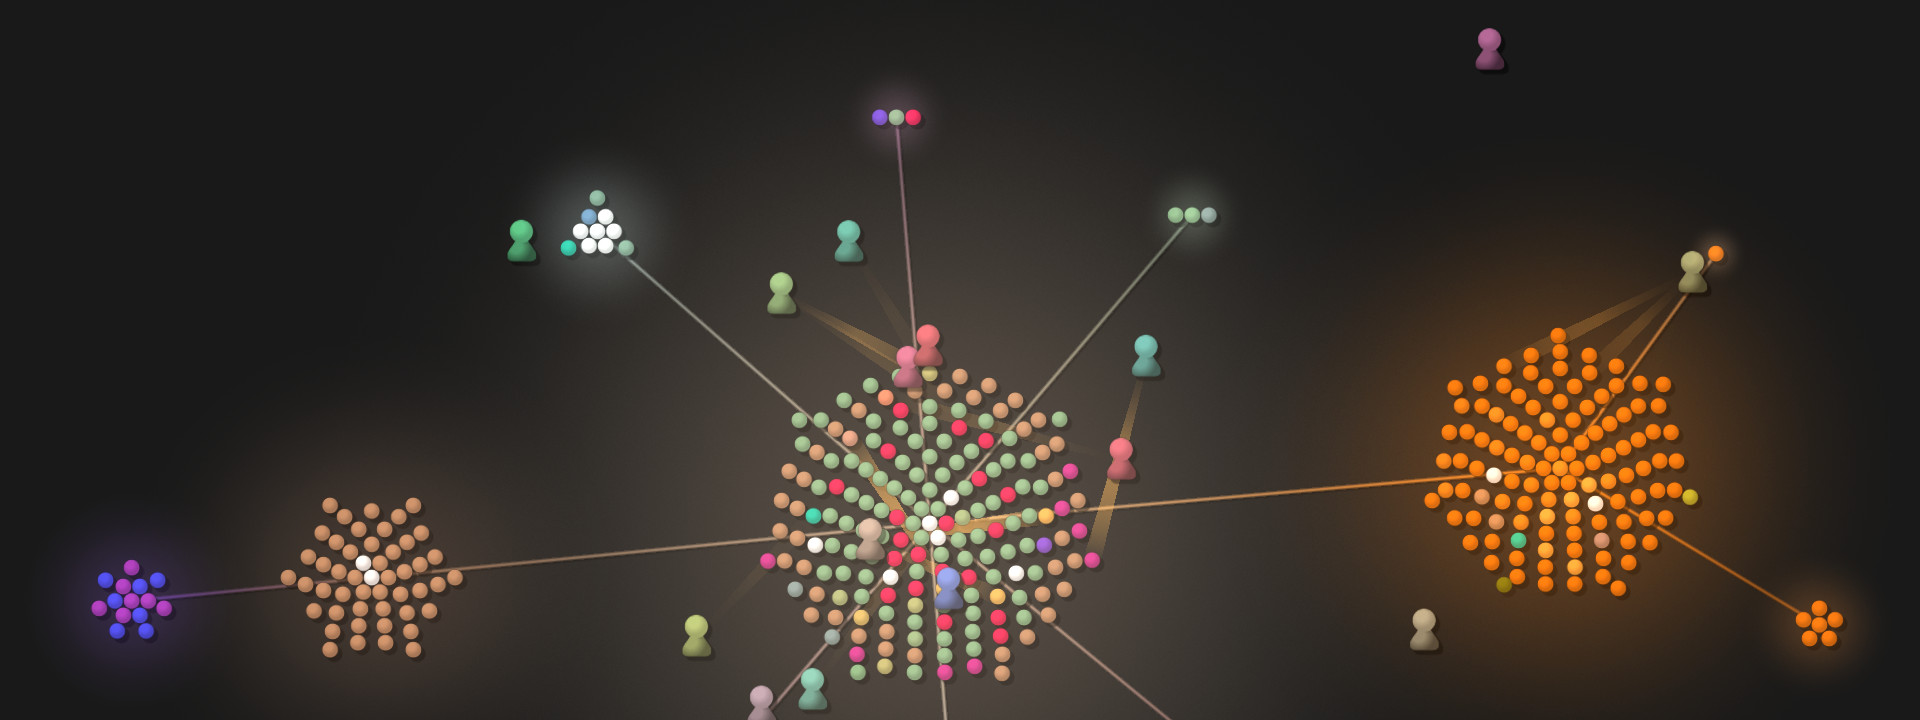
\includegraphics[scale=0.2]{Gambar/gource.jpg}
	\caption{Visualisasi proyek perangkat lunak menggunakan Gource.}
	\label{fig:gource}
\end{figure}

Gambar \ref{fig:gource} menunjukkan contoh visualisasi proyek perangkat lunak menggunakan Gource. Gource dapat digunakan untuk membuat visualisasi perkembangan proyek perangkat lunak, mulai dari awal perkembangan sampai akhir. Pada awalnya ukuran \textit{working tree} tidak terlalu besar. Setiap kali ditambahkan \textit{file} dan \textit{folder} baru, akan dibuat \textit{branch} dan \textit{leaf} baru pada \textit{working tree}.

Terdapat beberapa fitur penting pada Gource. Gource dapat menampilkan judul dari proyek di pojok kiri bawah. Selain itu waktu animasi dapat ditampilkan di bagian atas. Gource dapat menampilkan \textit{caption} pada saat seorang \textit{developer} menambahkan \textit{file} atau \textit{folder}. \textit{Caption} ini berisi \textit{timestamp} dan deskripsi dari \textit{caption}. Animasi yang ditampilkan dapat diatur periode waktunya.  
 
 \section{Analisis Penggunaan Git Command Line}
\label{sec:analisis_git}

Terdapat dua permasalahan dalam skripsi ini. Permasalahan pertama membahas tentang cara membangkitkan animasi \textit{timelapse} pada pengembangan proyek perangkat lunak berbasis web. Permasalahan kedua membahas tentang cara mengimplementasikan aplikasi tersebut. Pada bab ini akan dibahas analisis penggunaan beberapa \textit{library} untuk membuat animasi \textit{timelapse}. Proyek perangkat lunak yang digunakan pada bab ini adalah Piktora\footnote{http://piktora.com}. 

Git Command Line dapat digunakan untuk berinteraksi dengan repositori yang terekam oleh Git. Git Command Line dapat menjalankan perintah-perintah Git(lihat \ref{subsec:operasi_dasar_git}). Histori \textit{commit} dapat didapatkan dengan menggunakan operasi Git Log. Sintaks untuk menjalankan operasi Git Log adalah \texttt{\$ git log}. Listing \ref{lst:commit_history_piktora} menunjukkan sebagian histori \textit{commit} dari proyek Piktora. Pada histori \textit{commit} dapat dilihat \textit{author} dari yang melakukan \textit{commit} beserta \textit{email}nya, tanggal dan waktu dilakukan \textit{commit}, deskripsi \textit{commit}, dan nilai SHA-1 sepanjang 40 bit. 

\begin{lstlisting}[caption={Histori \textit{commit} pada proyek Piktora},label={lst:commit_history_piktora},language=plaintext]
C:\xampp\htdocs\Piktora>git log
commit 89000be7ce7d16f006813cddefb4ec6d70d15ed6 (HEAD -> master, origin/master, origin/HEAD)
Author: Hizkia Steven <xvii.hs@gmail.com>
Date:   Fri Jan 12 12:25:30 2018 +0700

    Update new company address

commit 6a085c1c37949e6308cfe06a117302e528388e54
Author: Hizkia Steven <xvii.hs@gmail.com>
Date:   Tue Dec 12 14:38:38 2017 +0700

    Update company address

commit 9f041ef239bfe236ab4d679ad698d773a8ba6f56
Author: TommyAdhityaThe <toms.warior@gmail.com>
Date:   Mon May 15 10:40:16 2017 +0700

    set insta url to https://www.instagram.com/piktorastudio/

commit 38711f0cc8f487aac62babac10c1185f5ee14d33
Author: Tommy Adhitya The <toms.warior@gmail.com>
Date:   Mon Apr 17 15:15:03 2017 +0700

    fix bug ugly display when projects too high

commit 9bfde3ceffc622f99e2e73cd1c9263fef72bc5b9
Author: Tommy Adhitya The <toms.warior@gmail.com>
Date:   Mon Apr 17 15:09:54 2017 +0700

    add ignore sftp-config.json

commit 18c39ef4ad68b3ad503bc13a788d3979e04ec3f9
Author: Pascal Alfadian Nugroho <pascalalfadian@live.com>
Date:   Thu Apr 13 15:21:49 2017 +0700

    Test commit (in gitlab). Nothing much important

commit 33702c2c674bb2dbb16dac1827b49af21969f24f
Author: Tommy Adhitya The <toms.warior@gmail.com>
Date:   Tue Feb 21 13:31:08 2017 +0700

    change email sender to piktora@mailgun.dnartworks.com.au
    
\end{lstlisting}
\ \\

Histori \textit{commit} ditampilkan berdasarkan urutan waktu dilakukannya \textit{commit}. Pada listing \ref{lst:commit_history_piktora}, histori \textit{commit} ditampilkan mulai dari \textit{commit} terbaru hingga \textit{commit} terlama. Listing \ref{lst:commit_history_piktora} menampilkan \textit{commit} pada tanggal 12 Januari 2018, kemudian tanggal 12 Desember 2017, kemudian tanggal 15 Mei 2017, dst. Histori \textit{commit} juga dapat ditampilkan mulai dari \textit{commit} terlama hingga \textit{commit} terbaru. Perintah untuk menampilkan urutan \textit{commit} berdasarkan urutan terlama adalah \texttt{\$ git log --reverse}. Listing \ref{lst:commit_history_piktora_reverse} menunjukkan histori \textit{commit} pada tanggal 31 Oktober 2016, kemudian 5 November 2016, dst. 

\begin{lstlisting}[caption={Histori \textit{commit} pada proyek Piktora, ditampilkan dengan urutan \textit{commit} terlama},label={lst:commit_history_piktora_reverse},language=plaintext]
C:\xampp\htdocs\Piktora>git log --reverse
commit 315d37462467f7aaa2c9e6c7a200c176e96ce5b4
Author: Pascal Alfadian Nugroho <pascalalfadian@live.com>
Date:   Mon Oct 31 16:52:46 2016 +0700

    Basic CI files + htaccess & webconfig + database.php ignore

commit 27ce3d4a22d95e0b5fbb7ecdfb8c863cdb53e895
Author: Tommy Adhitya The <toms.warior@gmail.com>
Date:   Sat Nov 5 13:12:43 2016 +0700

    setup environment for piktora

commit 65f0c9c59ac8cb9e7d572ab7a8fa91fe05232274
Author: Tommy Adhitya The <toms.warior@gmail.com>
Date:   Sat Nov 5 19:22:58 2016 +0700

    * create structure for all pages
    * add dummy images

commit bffbae1b0fb2cbea6b66ef9699d666faf66a03a4
Author: Tommy Adhitya The <toms.warior@gmail.com>
Date:   Tue Nov 8 18:00:32 2016 +0700

    - basic structure (navbar semi complete)
    - add fonts

commit 5c59916009bc47748b0fc2398d12ef532417548f
Author: Tommy Adhitya The <toms.warior@gmail.com>
Date:   Tue Nov 8 19:51:18 2016 +0700

    implement navbar, footer, and projects/ page

commit 77383808cd2717e1debcc75a057d414bd3135c18
Author: Tommy Adhitya The <toms.warior@gmail.com>
Date:   Tue Nov 8 20:05:27 2016 +0700

    fix pc and ipad navbar fontsize

commit 26bdbeebd42813cb2bb5f87291e4597efd221d41
Author: Tommy Adhitya The <toms.warior@gmail.com>
Date:   Tue Nov 8 20:16:33 2016 +0700

    fix position image for desktop /projects
    
\end{lstlisting}
\ \\
Untuk dapat berpindah ke \textit{commit} tertentu digunakan operasi Git Checkout. Dengan menggunakan operasi Git Checkout, dapat dilihat \textit{state} dari \textit{file-file} pada \textit{commit} tertentu. Sintaks untuk menjalankan perintah Git Checkout pada Git Command Line adalah \texttt{\$ git checkout [SHA-1 commit]}. Dimana parameternya adalah nilai dari SHA-1 suatu \textit{commit}. SHA-1 mempunyai panjang 40 bit, tetapi cukup 7 bit pertama saja yang dimasukkan ke parameter.

\begin{lstlisting}[caption={Git Checkout ke \textit{commit} pertama pada proyek Piktora},label={lst:checkout_piktora},language=plaintext]
C:\xampp\htdocs\Piktora>git checkout 315d374
Checking out files: 100% (5583/5583), done.
Note: checking out '315d374'.

You are in 'detached HEAD' state. You can look around, make experimental
changes and commit them, and you can discard any commits you make in this
state without impacting any branches by performing another checkout.

If you want to create a new branch to retain commits you create, you may
do so (now or later) by using -b with the checkout command again. Example:

  git checkout -b <new-branch-name>

HEAD is now at 315d374 Basic CI files + htaccess & webconfig + database.php ignore    
\end{lstlisting}
\ \\   
Listing \ref{lst:checkout_piktora} menunjukkan operasi \textit{checkout} ke \textit{commit} pertama pada proyek Piktora.  Nilai SHA-1 dari \textit{commit} pertama didapatkan pada listing \ref{lst:commit_history_piktora_reverse}, dimana hanya 7 bit pertama saja yang diambil. Baris ke-5 menunjukkan bahwa HEAD dalam keadaan \textit{DETACHED}(lihat \ref{subsec:git_checkout}). Baris ke-14 memperlihatkan bahwa HEAD sedang menunjuk pada \textit{commit} pertama.

\begin{figure}[H]
	\centering
		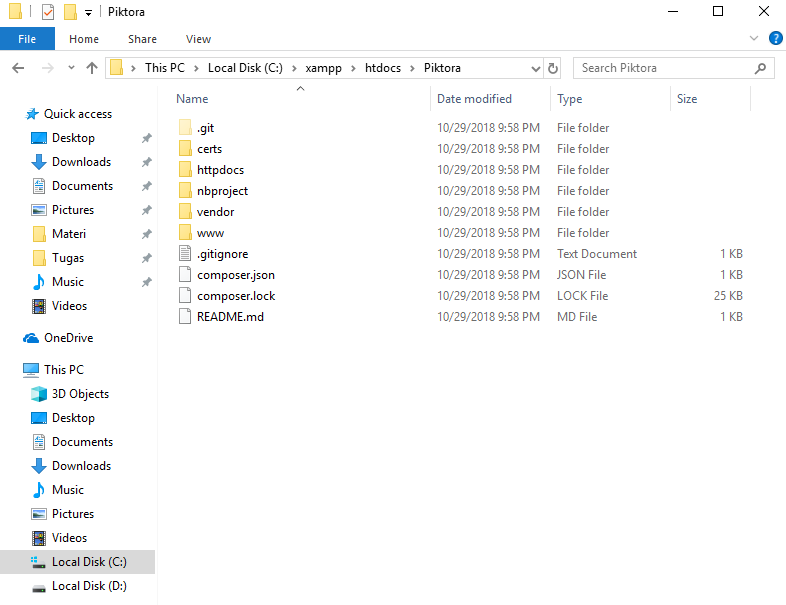
\includegraphics[scale=0.6]{Gambar/piktora_last_commit.png}
	\caption{\textit{Working tree} proyek Piktora pada \textit{commit} terakhir.}
	\label{fig:piktora_last_wt}
\end{figure}
\ \\
Gambar \ref{fig:piktora_last_wt} menunjukkan \textit{working tree} proyek Piktora pada \textit{commit} terakhir. \textit{Folder} git menunjukkan bahwa direktori Piktora terekam oleh Git. \textit{File} dan \textit{folder} yang terdapat pada \textit{working tree} merupakan \textit{snapshot} dari suatu\textit{commit}. Setiap kali dilakukan \textit{checkout}, \textit{working tree} akan berubah sesuai dengan \textit{snapshot} pada \textit{commit} tertentu. Dengan menggunakan operasi \textit{checkout}, dapat dibandingkan \textit{file} versi sekarang dengan \textit{file} pada versi sebelumnya.    
\begin{figure}[H]
	\centering
		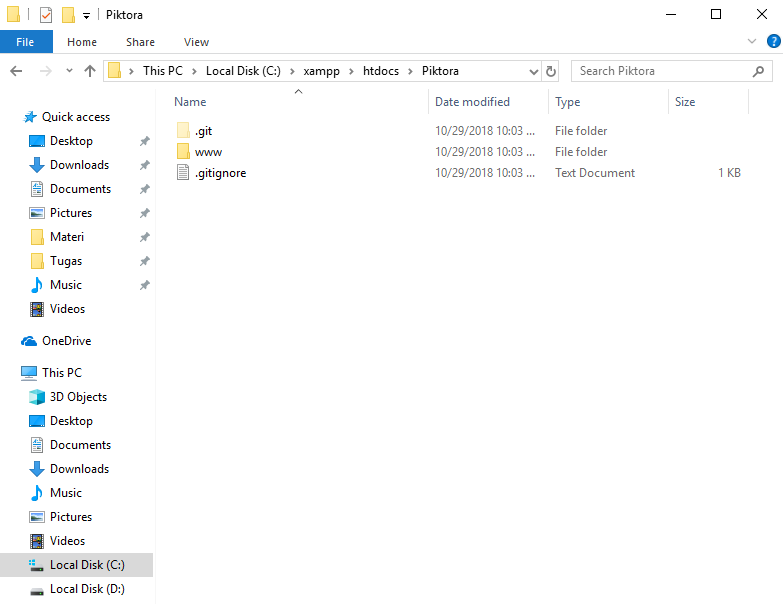
\includegraphics[scale=0.6]{Gambar/piktora_first_commit.png}
	\caption{\textit{Working tree} proyek Piktora pada \textit{commit} pertama.}
	\label{fig:piktora_first_wt}
\end{figure}
\ \\
Gambar \ref{fig:piktora_first_wt} menunjukkan \textit{working tree} proyek Piktora setelah dilakukan \textit{checkout} ke  \textit{commit} pertama. Jika dilihat, terdapat perbedaan \textit{working tree} antara \textit{commit} pertama dan terakhir. Pada \textit{commit} pertama, \textit{working tree} hanya berisi \textit{folder} git, \textit{folder} www, dan \textit{file} file gitignore.  Pada \textit{commit} terakhir, terdapat beberapa \textit{file} dan \textit{folder} baru di \textit{working tree}. 
 
\begin{figure}[H]
	\centering
		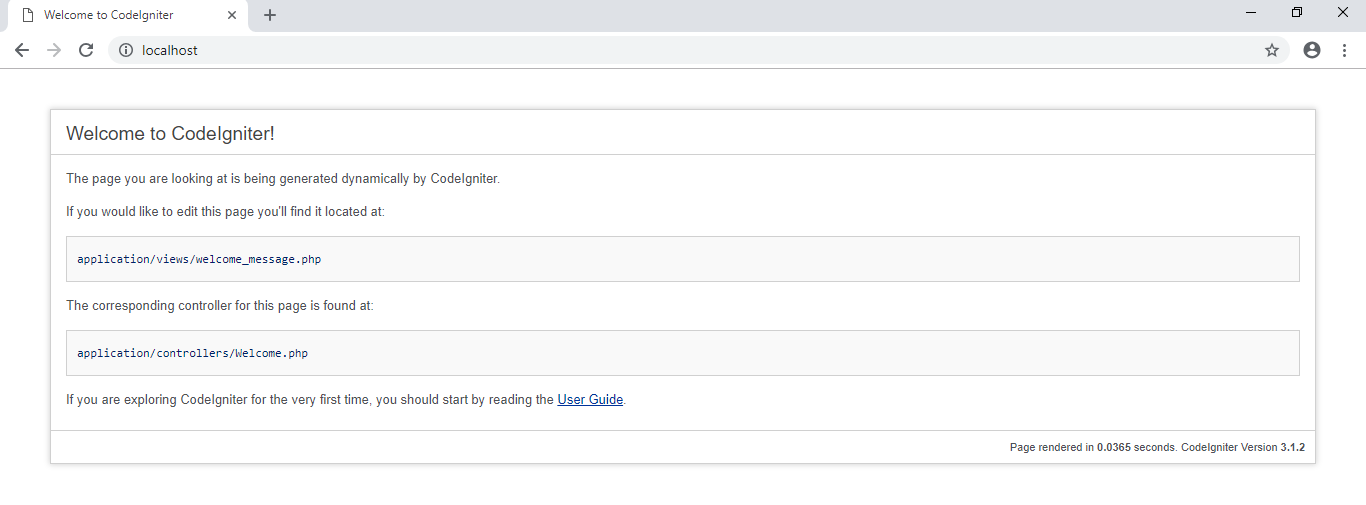
\includegraphics[scale=0.5]{Gambar/piktora_versi_pertama.png}
	\caption{Halaman \textit{web} proyek Piktora pada \textit{commit} pertama.}
	\label{fig:piktora_web_first}
\end{figure} 
\ \\
Selain terdapat perbedaan di \textit{working tree}, terdapat juga perbedaan pada halaman \textit{web} versi pertama dan terakhir. Gambar \ref{fig:piktora_first_wt} menunjukkan halaman \textit{web} Piktora pada \textit{commit} pertama. Gambar \ref{fig:piktora_last_wt} menunjukkan halaman \textit{web} Piktora pada \textit{commit} terakhir.
\begin{figure}[H]
	\centering
		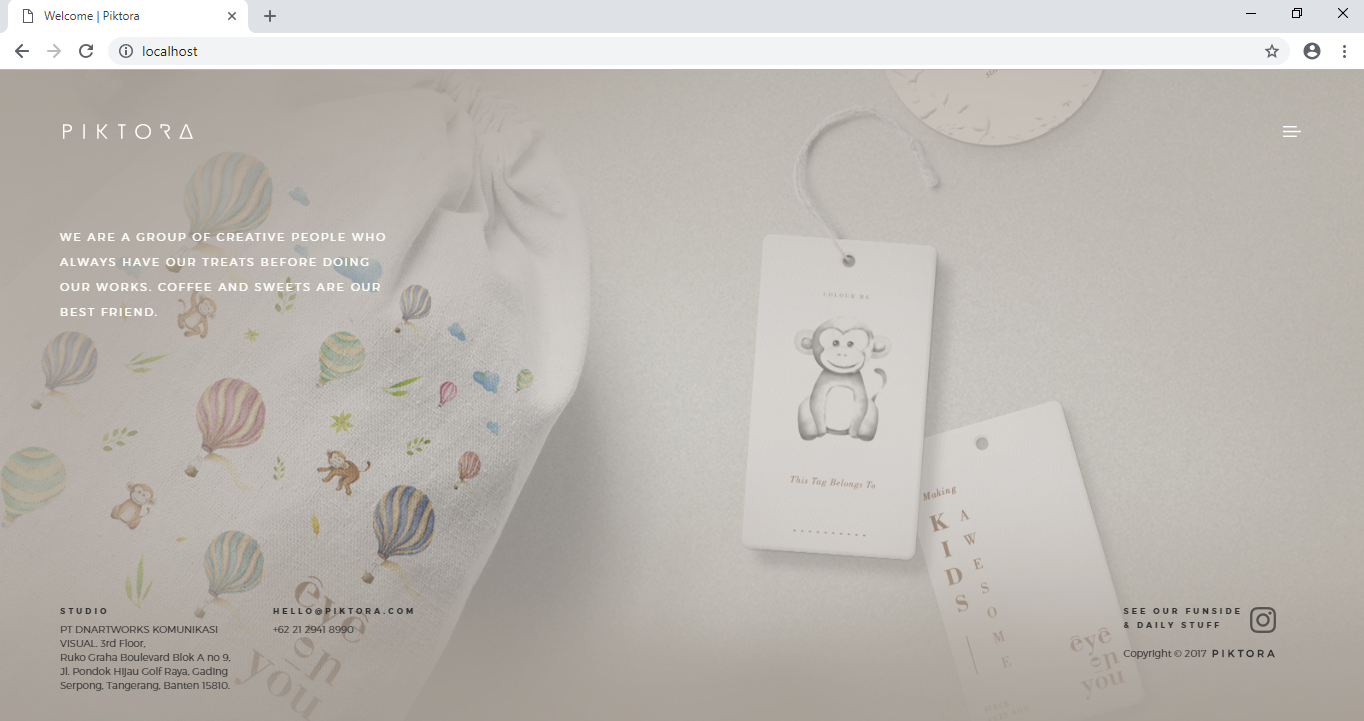
\includegraphics[scale=0.5]{Gambar/piktora_versi_terakhir.png}
	\caption{Halaman \textit{web} proyek Piktora pada \textit{commit} terakhir.}
	\label{fig:piktora_web_last}
\end{figure} 


%\section{Analisis Penggunaan JGit}
%\label{sec:analisis_jgit}


%\section{Analisis Penggunaan Selenium WebDriver}
%\label{sec:analisis_selenium}

%\section{Analisis Penggunaan Apache Commons CLI}
%\label{sec:analisis_apache_commons}

\section{Prapengujian}
\label{sec:prapengujian}
Pen




